\documentclass[letterpaper,11pt]{report}
% Change margins to 1 inch on all sides
\addtolength{\oddsidemargin}{-.875in}
\addtolength{\evensidemargin}{-.875in}
\addtolength{\textwidth}{1.75in}
\addtolength{\topmargin}{-.875in}
\addtolength{\textheight}{1.75in}
\usepackage{float}
\usepackage{graphicx}
\usepackage{footnote}
\usepackage{longtable}
\usepackage{multirow}
\usepackage{tablefootnote}
\usepackage{tabularx}
\usepackage{url}
\DeclareGraphicsExtensions{.pdf,.png,.jpg}

%%%%%%%%%%Start of report
\begin{document} 
\begin{savenotes}
\pagestyle{plain}
\title{CS896 Introduction to Web Science\\Fall 2013\\Report for Assignment 6}
\author{Corren G. McCoy}
 
\date{October 31, 2013}
\maketitle

\renewcommand*\thesection{\arabic{section}}
\setcounter{section}{0}

\setcounter{tocdepth}{4}
\tableofcontents
 \listoffigures
 \listoftables
\newpage


%%%%%%%%%%Chapter Exercises
\section{Question 1}
\subsection{Problem}We know the result of the Karate Club (Zachary, 1977)\cite{zachary1977information} split. Prove or disprove that the result of split could have been predicted by the weighted graph of social interactions. How well does the mathematical model represent reality? Generously document your answer with all supporting equations, code, graphs, arguments, etc.
\subsection{Response}We will proceed with a direct proof to determine whether a logical sequences of steps can reasonably generate the desired community structure. We are given the final network structure shown in Figure \ref{fig:zachary} which identifies membership in the two clubs after the division by the shaded and unshaded nodes. Even though the two groups are very interconnected, we must determine whether the structure itself provides enough information to predict the division between the group members.

\begin{figure}[htbp]
	\centering
		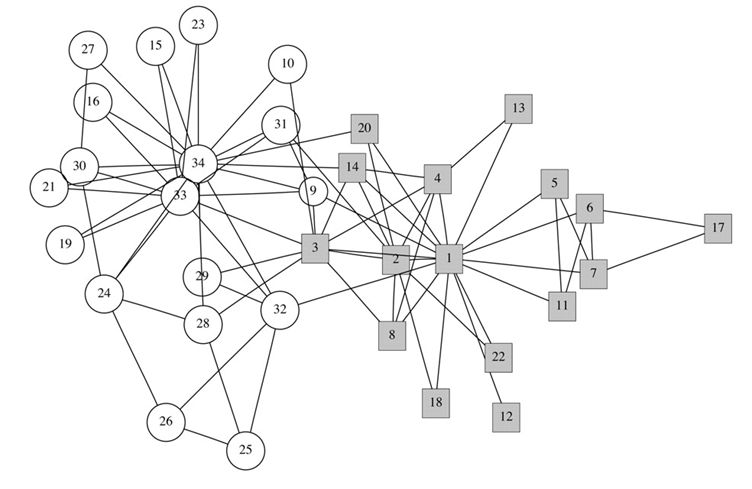
\includegraphics[width=1.00\textwidth]{zachary.png}
	\caption{Zachary Karate Club}
	\label{fig:zachary}
\end{figure}

\subsection{Methodology}To properly identify the division in the karate club, we need to carefully examine the edges between the groups. For the analysis of the graph partitions, we will employ a divisive method proposed by Girvan and Newman \cite{girvan2001community}. This method defines an abstract concept of traffic on the network and looks for the edges that carry the most of this traffic. For each pair of nodes A and B in the graph that are connected, we calculate the flow along the edges. Girvan-Newman defines the betweenness of an edge to be the total amount of flow it carries when considering all pairs of nodes using this edge.  Now, based on the premise that the nodes with high traffic are the most vital edges for connecting different regions of the network, the algorithm tries to remove these nodes first. The basic idea of this method is that two communities should be connected by edges that operate as bridges, through which the traffic should be relatively high. Therefore, by ranking all edges according to their betweenness and then removing the edges with the largest value, we should obtain community partitions. By iteratively recalculating betweenness, we can implement a divisive algorithm for detecting community structure in the undirected graph. This concept is the underlying premise of the Girvan-Newman method which is summarized using the following steps:

\begin{enumerate}
\item First, calculate the betweenness of all existing edges in the network. For any given node, compute the total flow along the shortest path from that node to all others.
\item The edge with the highest betweenness is removed. If there is a tie, remove both edges from the graph. 
\item The betweenness of all edges affected by the removal is recalculated.
\item Repeat steps 2 and 3 until either no edges remain or the desired number of communities is obtained.
\end{enumerate}

To apply the algorithm, we used the weighted graph representation of the karate club which is available in the igraphdata\footnote{\url{http://cran.r-project.org/web/packages/igraphdata/igraphdata.pdf}} package in ``R''. The data in this package is the same as the quantified matrix of social interactions defined in Zachary's\cite{zachary1977information} Figure 3. For reference, the same figure is included here in Appendix \ref{chap:fig3}. To apply the Girvan-Newman method, we implemented a function in ``R'' which performs the following tasks:

\begin{itemize}
\item Accepts a parameter for the desired number of communities. The default is two;
\item Loads the karate club data into a graph object;
\item Applies the edge.betweenness.community\footnote{\url{http://www.inside-r.org/packages/cran/igraph/docs/edge.betweenness.community}} algorithm to the graph object;
\item Plots the graph object and highlights the top three candidates for removal;
\item Removes the edge with the highest value for betweenness;
\item Calculates modularity on the resulting network; and
\item Continues processing until either all edges are removed or the desired number of communities is obtained.
\end{itemize}

\indent{}The source code for the function is shown in Appendix \ref{chap:R}. The associated plot for each iteration of the algorithm is shown in Table \ref{tab:GirvanNewmanCommunityDetection}. When viewed from left to right, we see the edge with the highest level of betweenness is highlighted in red. The subsequent plot shows the impact of this edge's removal on the graph and the recalculation of betweenness. The final plot in the series shows a definitive separation of the graph into two distinct communities. 

\begin{table}[htbp]
	\centering
		\begin{tabular}{ccc}
			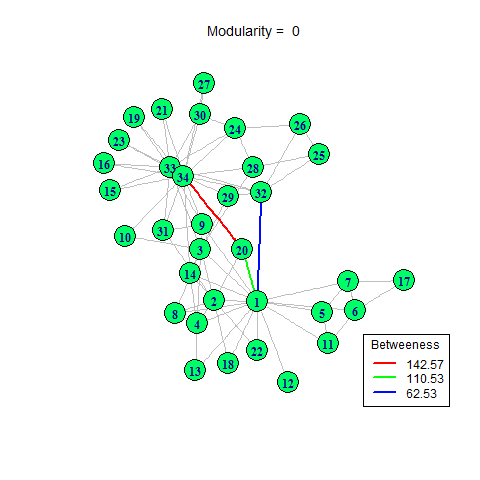
\includegraphics[scale=0.25]{karateClub-community-0001.png} &
			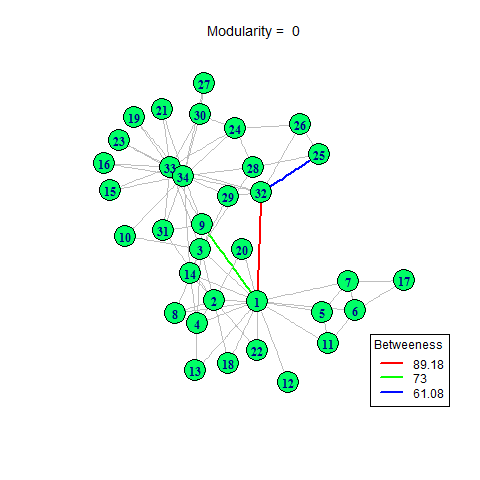
\includegraphics[scale=0.25]{karateClub-community-0002.png} & 
			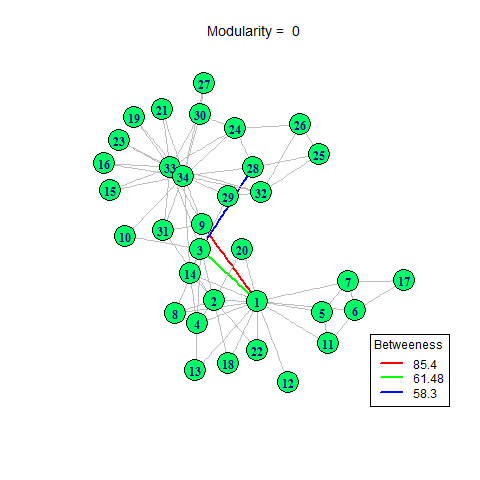
\includegraphics[scale=0.25]{karateClub-community-0003.png} \\
			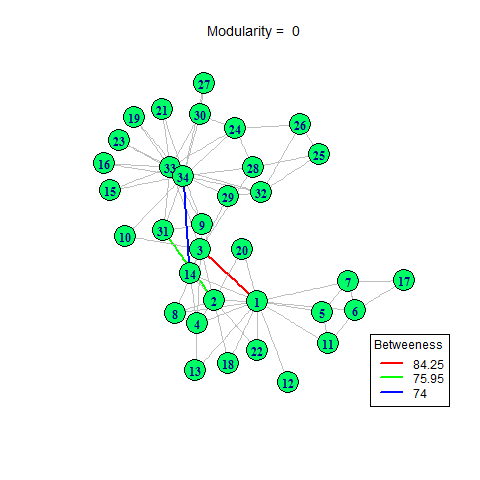
\includegraphics[scale=0.25]{karateClub-community-0004.png} &
			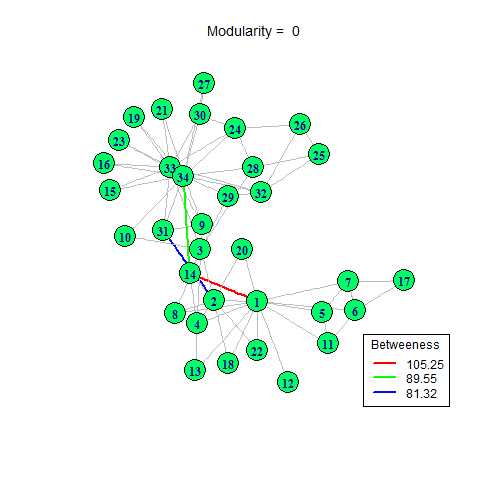
\includegraphics[scale=0.25]{karateClub-community-0005.png} & 
			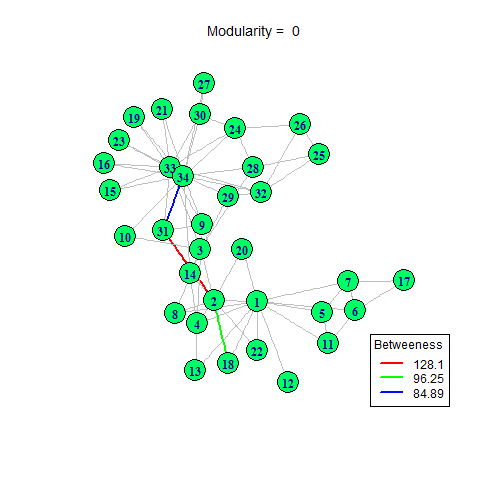
\includegraphics[scale=0.25]{karateClub-community-0006.png} \\
			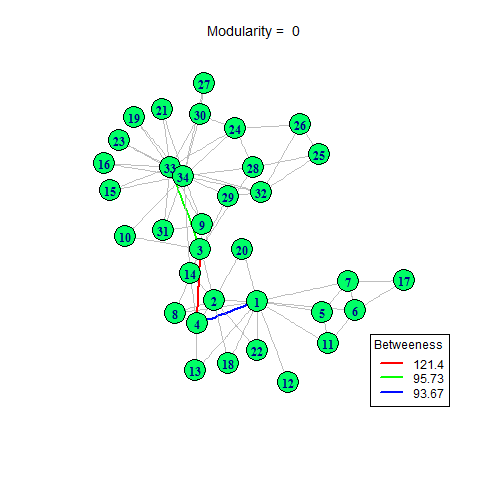
\includegraphics[scale=0.25]{karateClub-community-0007.png} &
			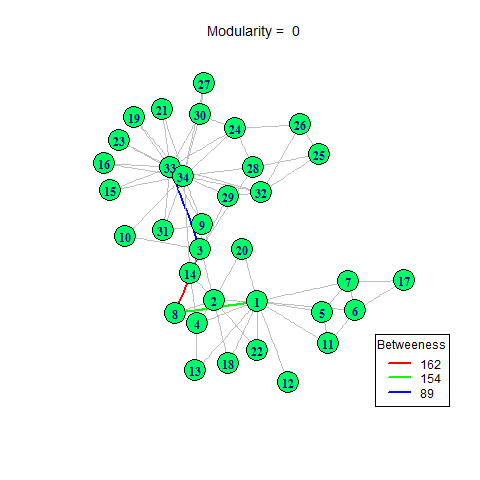
\includegraphics[scale=0.25]{karateClub-community-0008.png} & 
			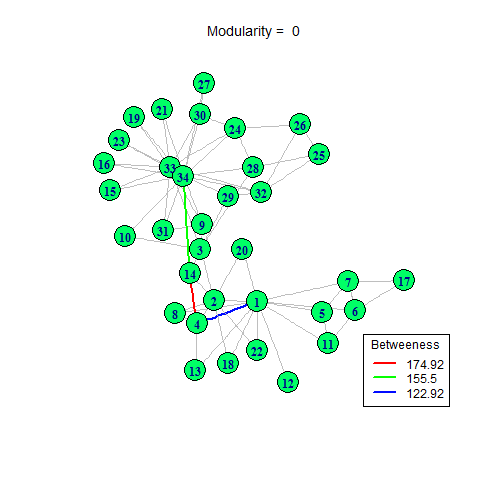
\includegraphics[scale=0.25]{karateClub-community-0009.png} \\
			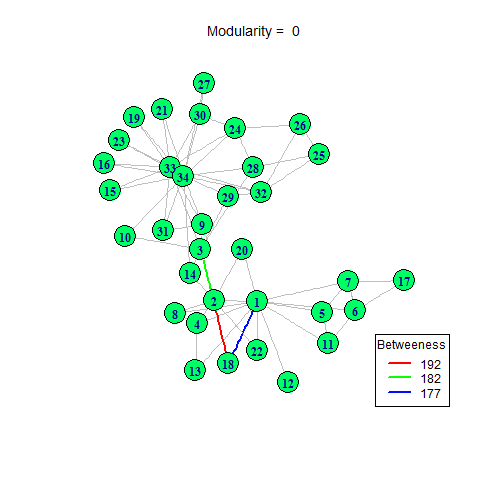
\includegraphics[scale=0.25]{karateClub-community-0010.png} &
			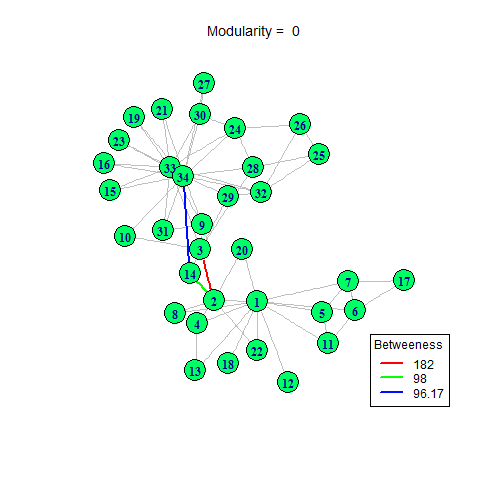
\includegraphics[scale=0.25]{karateClub-community-0011.png} & 
			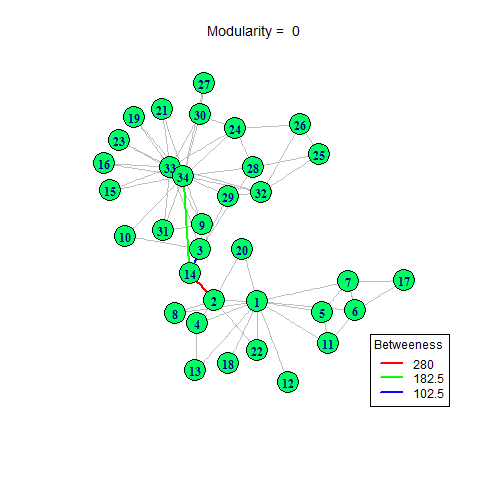
\includegraphics[scale=0.25]{karateClub-community-0012.png} \\
			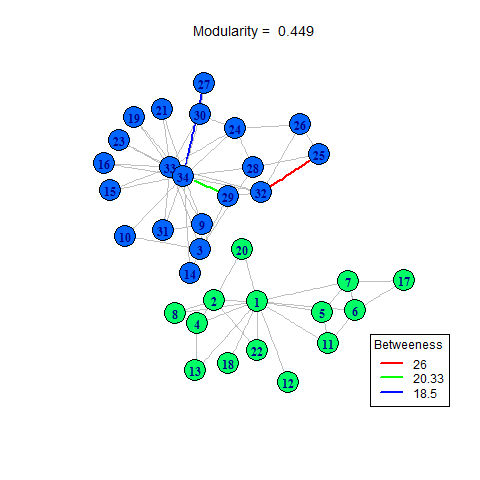
\includegraphics[scale=0.25]{karateClub-community-0013.png} &
			&  \\
		\end{tabular}
	\caption{Girvan-Newman Community Detection}
	\label{tab:GirvanNewmanCommunityDetection}
\end{table}

\indent{}Table \ref{tab:Evaluation} shows a comparison of the nodes in each cluster using Girvan-Newman to the known structure in Figure \ref{fig:zachary}. In the graph, node 1 is the instructor, Mr. Hi, while node 34 is the student officer. Three discrepancies in the assignments are noted with members 3, 9 and 14. The graph theory cannot predict subjective behavior or the affect of outside influences that cannot be measured. In this case, we know that the student represented by node 9 joined the instructor's club because he was only a few weeks away from obtaining his black belt. To join the officer's club, as suggested by the graph, would have meant starting over; thereby forfeiting three years of training. No exceptional circumstances were noted for members 3 and 14. Despite these small discrepancies, the Girvan-Newman algorithm achieved a 91\% hit ratio in assigning members to their respective community.

\begin{table}
    \begin{tabular}{|l|l|l|l|}
    \hline
    Member \#          & Zachary's After Split & Our Model & Hit / Miss         \\ \hline
    1                  & Mr. Hi                & Mr. Hi    & Hit                \\ \hline
    2                  & Mr. Hi                & Mr. Hi    & Hit                \\ \hline
    3                  & Mr. Hi                & Officer   & Miss*               \\ \hline
    4                  & Mr. Hi                & Mr. Hi    & Hit                \\ \hline
    5                  & Mr. Hi                & Mr. Hi    & Hit                \\ \hline
    6                  & Mr. Hi                & Mr. Hi    & Hit                \\ \hline
    7                  & Mr. Hi                & Mr. Hi    & Hit                \\ \hline
    8                  & Mr. Hi                & Mr. Hi    & Hit                \\ \hline
    9                  & Mr. Hi                & Officer   & Miss*               \\ \hline
    10                 & Officer               & Officer   & Hit                \\ \hline
    11                 & Mr. Hi                & Mr. Hi    & Hit                \\ \hline
    12                 & Mr. Hi                & Mr. Hi    & Hit                \\ \hline
    13                 & Mr. Hi                & Mr. Hi    & Hit                \\ \hline
    14                 & Mr. Hi                & Officer   & Miss*               \\ \hline
    15                 & Officer               & Officer   & Hit                \\ \hline
    16                 & Officer               & Officer   & Hit                \\ \hline
    17                 & Mr. Hi                & Mr. Hi    & Hit                \\ \hline
    18                 & Mr. Hi                & Mr. Hi    & Hit                \\ \hline
    19                 & Officer               & Officer   & Hit                \\ \hline
    20                 & Mr. Hi                & Mr. Hi    & Hit                \\ \hline
    21                 & Officer               & Officer   & Hit                \\ \hline
    22                 & Mr. Hi                & Mr. Hi    & Hit                \\ \hline
    23                 & Officer               & Officer   & Hit                \\ \hline
    24                 & Officer               & Officer   & Hit                \\ \hline
    25                 & Officer               & Officer   & Hit                \\ \hline
    26                 & Officer               & Officer   & Hit                \\ \hline
    27                 & Officer               & Officer   & Hit                \\ \hline
    28                 & Officer               & Officer   & Hit                \\ \hline
    29                 & Officer               & Officer   & Hit                \\ \hline
    30                 & Officer               & Officer   & Hit                \\ \hline
    31                 & Officer               & Officer   & Hit                \\ \hline
    32                 & Officer               & Officer   & Hit                \\ \hline
    33                 & Officer               & Officer   & Hit                \\ \hline
    34                 & Officer               & Officer   & Hit                \\ \hline
    Total (Actual)     & ~                     & ~         & 31 Hits 3 Misses   \\ \hline
    Total (Percentage) & ~                     & ~         & 91.2\% Hits 8.8\% Misses \\ \hline
    \end{tabular}
			\caption{Evaluation}
	\label{tab:Evaluation}
\end{table}

As a final step, we would like to also apply an objective measure of the quality of the community divisions we obtained.  Newman \cite{newman2004finding} defines modularity (Q) as one ``measure of the quality of a particular division of a network.'' In his analysis of complex networks, Arenas \cite{arenas2008analysis} explains further that ``the modularity of a given partition is the probability of having edges falling within modules in the network minus the expected probability in an equivalent (random) network with the same number of nodes.'' In other words, we want to determine if the model performed better than a random assignment. A larger value for modularity indicates a strong community structure. While modularity can have a range of -1 to +1, Newman \cite{newman2004finding} indicates that Q values ``typically fall in the range from about 0.3 to 0.7.  Higher values are rare.'' The modularity function which we invoked in ``R'' is defined by the following mathematical equation where \emph{e} is an edge and \emph{a} is an element of the matrix. Our final plot in Table \ref{tab:GirvanNewmanCommunityDetection} shows a maximized Q value of 0.449 which when combined with our high hit ratio does indicate that the mathematical model can reasonably predict the actual karate club split.
\begin{equation}
Q = \sum (e_{ij} - a^{2}_{i}) 
\end{equation}

%%%%%%%%%%Chapter Exercises
\section{Question 2 Extra Credit}
\subsection{Problem}We know the group split in two different groups.  Suppose the disagreements in the group were more nuanced -- what would the clubs look like if they split into groups of 3, 4, and 5?
\subsection{Response}For this question, we used the same methodology and ``R'' function as stated in question 1. We passed a parameter to the ``R'' function to indicate the desired number of communities.  The results are shown in Figures \ref{fig:karateClubThreeGroups}, \ref{fig:karateClubFourGroups} and \ref{fig:karateClubFiveGroups}. A strong community structure is evidenced by the high modularity values of 0.567, 0.597 and 0.658 respectively,

\begin{figure}[htbp]
	\centering
		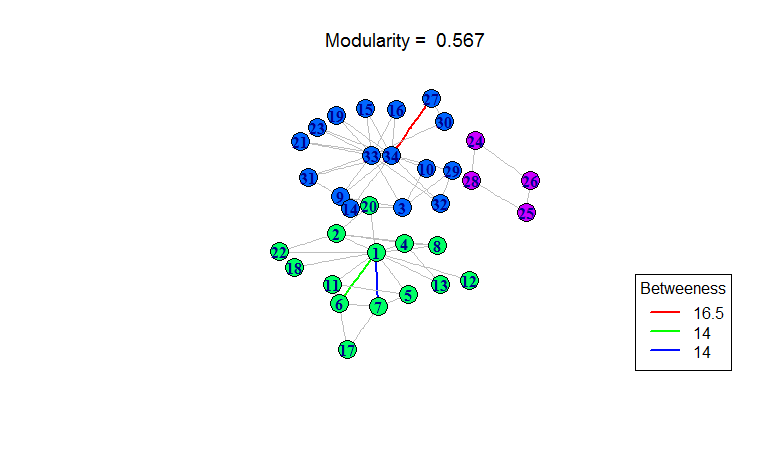
\includegraphics[width=1.00\textwidth]{karateClubThreeGroups.png}
	\caption{Karate Club - Three Groups}
	\label{fig:karateClubThreeGroups}
\end{figure}

\begin{figure}[htbp]
	\centering
		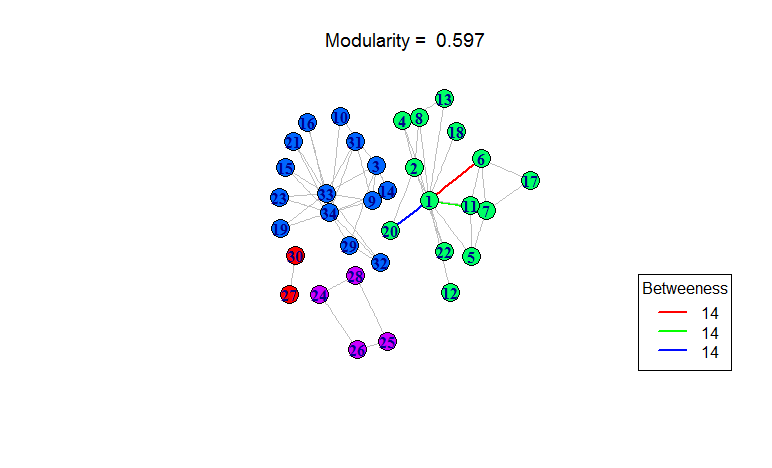
\includegraphics[width=1.00\textwidth]{karateClubFourGroups.png}
	\caption{Karate Club - Four Groups}
	\label{fig:karateClubFourGroups}
\end{figure}

\begin{figure}[htbp]
	\centering
		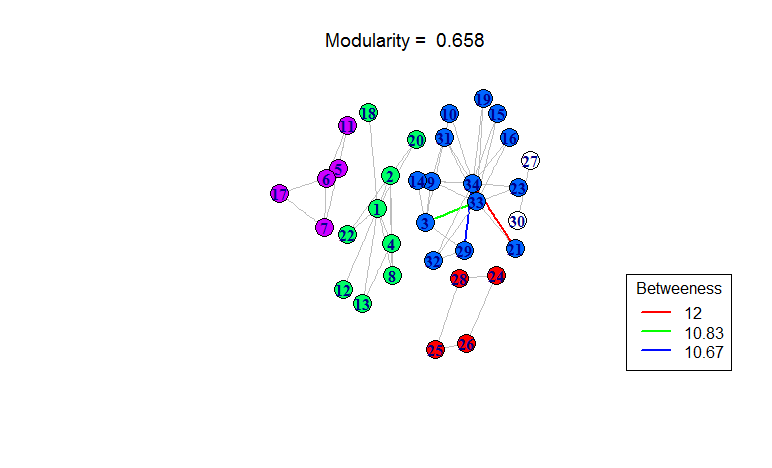
\includegraphics[width=1.00\textwidth]{karateClubFiveGroups.png}
	\caption{Karate Club - Five Groups}
	\label{fig:karateClubFiveGroups}
\end{figure}


\end{savenotes}

% produce the bibliography for the citations in your paper.
\bibliographystyle{abbrv}
\bibliography{cmccoy}

\appendix
\addcontentsline{toc}{chapter}{Appendices}

%%Appendix A
\chapter{``R'' Source Code} \label{chap:R}
\input{karateClub.r}
\chapter{Karate Club Quantified Matrix} \label{chap:fig3}
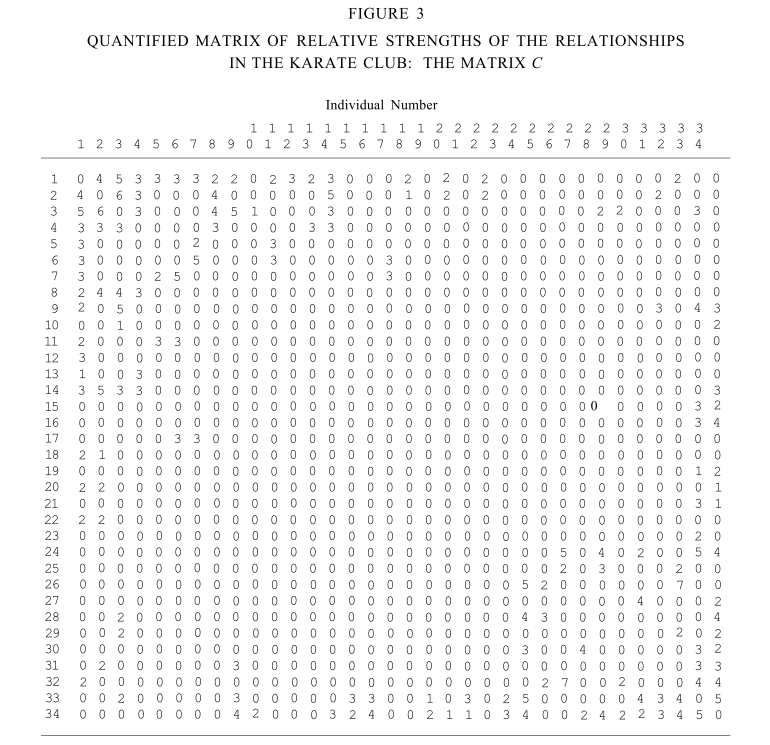
\includegraphics[width=1.00\textwidth]{ZacharyFigure3.png}
\end{document} 
%%%%%%%%%%Ed of report
